\documentclass[hidelinks,onefignum,onetabnum,final]{siamart220329}  % for arxiv
%\documentclass[review,hidelinks,onefignum,onetabnum,final]{siamart220329}  % for submission

\usepackage{amsfonts,yhmath}
\usepackage{graphicx}
\usepackage{epstopdf}
\ifpdf
  \DeclareGraphicsExtensions{.eps,.pdf,.png,.jpg}
\else
  \DeclareGraphicsExtensions{.eps}
\fi

% Used for creating new theorem and remark environments
\newsiamremark{remark}{Remark}
\newsiamremark{hypothesis}{Hypothesis}
\crefname{hypothesis}{Hypothesis}{Hypotheses}
\newsiamthm{claim}{Claim}
\newsiamthm{conjecture}{Conjecture}
\newsiamremark{example}{Example}

\usepackage{amsopn}
\DeclareMathOperator{\diag}{diag}

\usepackage{bm,bbm,empheq,verbatim,fancyvrb,amssymb}
\usepackage{booktabs,multirow,xspace}
\usepackage{pifont}

\usepackage{tikz}
\usetikzlibrary{decorations.pathreplacing}
\usetikzlibrary{graphs,quotes}

\newcommand{\eps}{\epsilon}
\newcommand{\RR}{\mathbb{R}}

\newcommand{\grad}{\nabla}
\newcommand{\Div}{\nabla\cdot}

\newcommand{\bbf}{\mathbf{f}}
\newcommand{\bg}{\mathbf{g}}
\newcommand{\bn}{\mathbf{n}}
\newcommand{\bu}{\mathbf{u}}
\newcommand{\bv}{\mathbf{v}}
\newcommand{\bw}{\mathbf{w}}
\newcommand{\bx}{\mathbf{x}}
\newcommand{\bz}{\mathbf{z}}

\newcommand{\bX}{\mathbf{X}}

\newcommand{\bzero}{\bm{0}}

\newcommand{\btau}{\bm{\tau}}

\newcommand{\cB}{\mathcal{B}}
\newcommand{\cH}{\mathcal{H}}
\newcommand{\cK}{\mathcal{K}}
\newcommand{\cV}{\mathcal{V}}

\newcommand{\hcK}{\widehat{\cK}}

\newcommand{\nn}{{\text{\textnormal{n}}}}
\newcommand{\pp}{{\text{\textnormal{p}}}}
\newcommand{\qq}{{\text{\textnormal{q}}}}
\newcommand{\rr}{{\text{\textnormal{r}}}}

\newcommand{\ip}[2]{\left<#1,#2\right>}

\newcommand{\XX}{\ding{55}}

\newcommand{\dx}{\, \mathrm{d}x}

\newcommand{\rhoi}{\rho_{\text{i}}}

\DeclareMathOperator*{\argmin}{arg\,min}
\DeclareMathOperator*{\Hull}{Hull}


% running headers and PDF metadata
\headers{Bounds on geometry errors in glacier simulations}{E. Bueler}

\title{Bounds on geometry errors in glacier simulations}

\author{Ed Bueler\thanks{Department of Mathematics and Statistics, University of Alaska Fairbanks, USA (\email{elbueler@alaska.edu}).}}


\begin{document}
\maketitle

\begin{abstract}
The primary data which determine the evolution of glaciation are bedrock elevation and surface mass balance.  From this data the glacier's geometry solves a free-boundary problem over a set of admissible surface elevation functions.  Admissibility requires that the ice surface elevation is above the bedrock topography, equivalently that the ice thickness is nonnegative.  For an implicit time step, the free-boundary problem can be posed in weak form as a variational inequality over a fixed map-plane region, and we conjecture that these continuous-space problems are well-posed in the case of non-shallow Stokes dynamics.  Then we show an abstract estimate for finite element approximations of variational inequality problems over Banach spaces, a theorem in which the nonlinear operator is assumed to be coercive and Lipshitz.  When applied in the glacier case, all terms in the error estimate can be physically-interpreted, and practical approaches to mitigate these errors are proposed.  The resulting computable bounds on the geometry approximation error are demonstrated in an implicit time-stepping glacier simulation based on Stokes dynamics.
\end{abstract}

% REQUIRED
\begin{keywords}
error bounds, finite element methods, glaciers, ice flow, variational inequalities
\end{keywords}

% REQUIRED
%\begin{MSCcodes}
%FIXME
%\end{MSCcodes}


\section{Introduction} \label{sec:intro}

Glacier and ice sheet simulations typically model the ice layer as a free-surface, very-viscous, incompressible, and non-Newtonian fluid \cite{GreveBlatter2009,SchoofHewitt2013}.  For simplicity we will restrict our considerations to simulations of glaciers on land, without floating portions, and we note that an ``ice sheet'' is simply a continent-scale glacier.

Two types of essential input data into such simulations are the bedrock elevation and the surface mass balance (SMB).  We will assume that the bedrock elevation map is constant in time.  By definition, the SMB is the annually-averaged difference of vertically-accumulating snow minus the loss of (liquid) water, through runoff, at the upper surface of the glacier \cite{Cogleyetal2011}, and we assume it depends on time.  Note that elevations are measured here in meters, while the SMB is measured in ice-equivalent units of meters per second.

Thus a glacier simulation takes an initial glacier geometry, the bedrock topography, and the time-dependent climate, i.e.~SMB, as inputs.  It produces the glacier's evolving geometry and flow velocity; these are the output fields of primary scientific value.  The geometry is parameterized by either the (upper) surface elevation or the ice thickness function.  The computed flow velocity is, however, only defined at those three-dimensional locations and times where ice is present, that is, on the evolving 3D domain between the bedrock and ice surface elevations.

Additional complications are common in comprehensive ice sheet models \cite{SchoofHewitt2013}, for example simulation of the internal energy of the ice \cite{Aschwandenetal2012}, and/or of the presence of liquid water within the ice matrix or at the glacier surfaces.  However, here we only consider conservation of mass and momentum, not energy, and furthermore we do not make the shallowness assumptions which are common in comprehensive models.

At a map-plane location and time where a glacier exists the surface elevation exceeds the bedrock elevation, equivalently the ice thickness is positive.  That is, the glacier's geometry must satisfy an inequality to be admissible.  Let $\Omega \subset \RR^2$ be a fixed portion of the earth's surface on which we are interested in glaciation (Figure \ref{fig:stokesdomain}), and let $x\in\Omega$ denote the map-plane coordinate(s).  Assume that we are given, as data, a bed elevation function $b(x)$ and an SMB function $a(t,x)$ for $t\in [0,T]$ and $x\in \Omega$.  (Function spaces for these data will be given below.)  Noting that $a$ is generally signed, in areas where $a>0$ (accumulation; downward arrows in Figure \ref{fig:stokesdomain}) then a glacier will exist, but if $a<0$ (upward arrows) then either a glacier exists with an ablating surface, or no glacier exists.  Determining which situation applies at a given $x\in\Omega$ requires solving a free-boundary problem.

\medskip
\begin{figure}[ht]
\centering
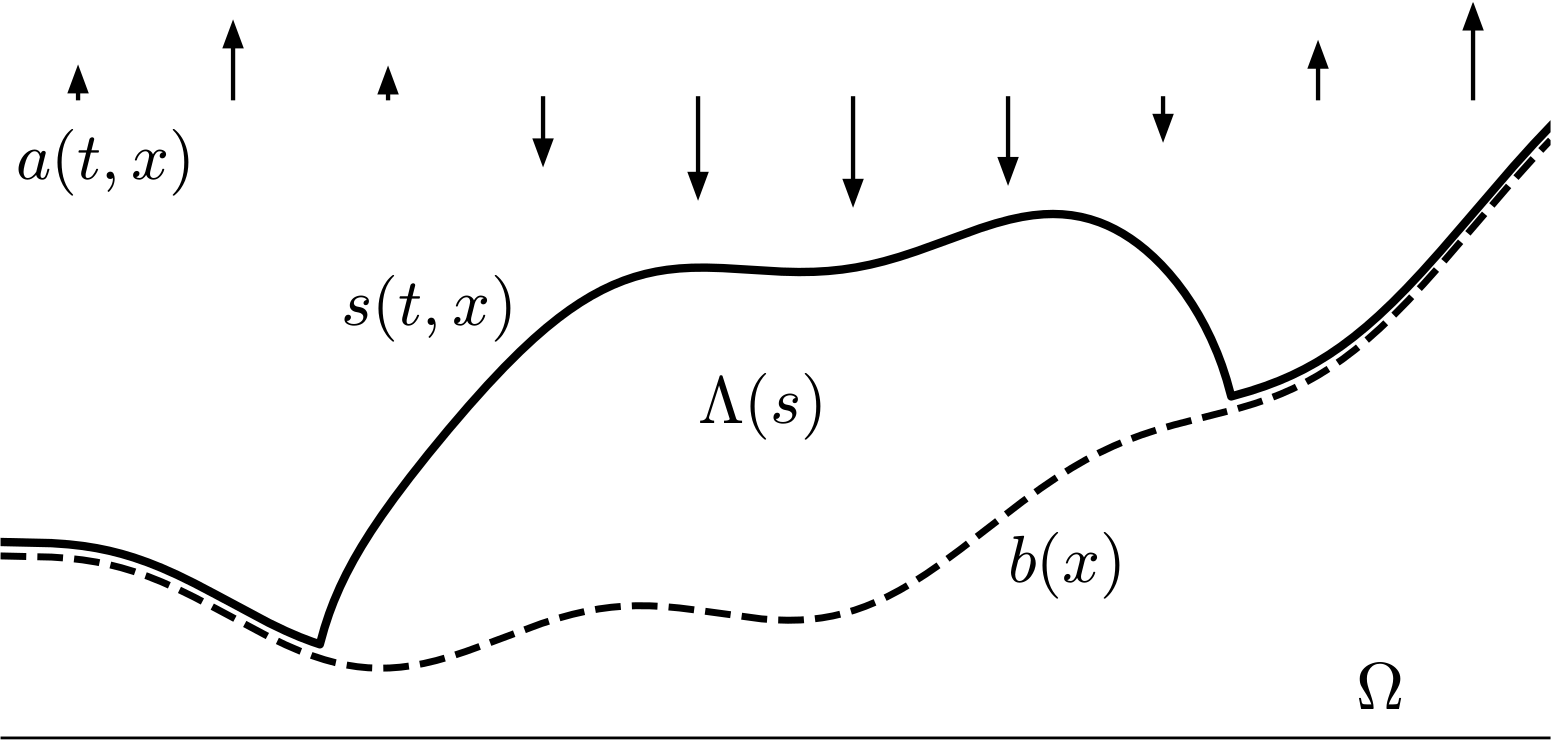
\includegraphics[width=0.65\textwidth]{genfigs/stokesdomain.pdf}
\caption{Glacier notation used in this paper.}
\label{fig:stokesdomain}
\end{figure}

\medskip
Let $s(t,x)$ be the (solution) ice surface elevation.  We will regard this as defined everywhere, but subject to the constraint that the surface $z=s(t,x)$ must be at or above the bedrock, $s(t,x) \ge b(x)$.  Note that some regions in $\Omega$ may have no ice $s(t,x)=b(x)$.  The solution ice velocity $\bu(t,x,z)$ and pressure $p(t,x,z)$ are then defined only on the 3D domain
\begin{equation}
\Lambda(t) = \left\{(x,z)\,:\,b(x) < z < s(t,x)\right\} \subset \Omega \times \RR. \label{eq:icydomain}
\end{equation}
This aspect of glacier modeling deserves emphasis: at any time $t$ the 3D domain $\Lambda(t)$, on which the velocity and pressure are meaningful, is determined by the time-dependent surface elevation $s(t,x)$ which is part of the solution.

Denote the surface value (trace \cite{Evans2010}) of the velocity solution by $\bu|_s$, and let $\bn_s = \left<-\grad s,1\right>$ be a 3D, un-normalized surface normal vector.  For any $T>0$, an infinite-dimensional nonlinear complementarity problem (NCP) \cite{Bueler2021conservation,FacchineiPang2003,SchoofHewitt2013} applies almost everywhere in $[0,T]\times \Omega$:
\begin{subequations}
\label{eq:ncp}
\begin{align}
s - b &\ge 0 \\
\frac{\partial s}{\partial t} - \bu|_s \cdot \bn_s - a &\ge 0 \\
(s - b) \left(\frac{\partial s}{\partial t} - \bu|_s \cdot \bn_s - a\right) &= 0
\end{align}
\end{subequations}
This strong form NCP statement, which will be reformulated as a variational inequality (VI; \cite{KinderlehrerStampacchia1980}) in Section \ref{sec:model} below, assumes that we have extended the surface velocity by zero ($\bu|_s=0$) to the ice-free areas where $s(t,x)=b(x)$.  This NCP says that either a location is ice free ($s-b=0$) and that the climate is locally ablating ($a<0$), or that the surface kinematical equation (SKE) holds:
\begin{equation}
\frac{\partial s}{\partial t} - \bu|_s \cdot \bn_s - a = 0.  \label{eq:ske}
\end{equation}

Well-known equation \eqref{eq:ske} states that the (non-material) surface of the ice moves vertically according to the sum of a component of the ice velocity at the surface and the SMB \cite{SchoofHewitt2013}.  This is a statement of mass conservation at a non-material surface \cite{Aschwandenetal2012}, sometimes wrongly\footnote{Equation \eqref{eq:ske} is not the boundary condition for any identifiable problem.} called a ``kinematical boundary condition'' \cite{GreveBlatter2009}.

The SMB $a(t,x)$ is assumed to be defined everywhere in $\Omega$, regardless of whether a glacier is present or not.  At an ice-free ablative location the value $a(t,x)\le 0$ can be modeled using precipitation and an energy balance \cite{GreveBlatter2009}, for instance by hypothesizing an ice or snow surface, and then computing the balance of snow accumulation versus the total runoff from the available energy for melt.  In other words, the provided SMB at an unglaciated location needs to give the value which a glacier would experience if it were present at that time and place.

Within the ice the simulation needs to conserve mass and momentum.  From \eqref{eq:icydomain} let $\Gamma_s(t) \subset \partial \Lambda(t)$ be the upper surface $z=s$ and
$\Gamma_b(t) \subset \partial \Lambda(t)$ be the base $z=b$.  The models considered here neglect the possibility of fracture-generated cliffs at the ice margin, so we assume $\partial \Lambda(t) = \overline{\Gamma_s(t)} \cup \overline{\Gamma_b(t)}$ at any time.  To conserve mass and momentum within the ice we assume the standard non-shallow ice dynamics model, namely a non-Newtonian and incompressible Stokes problem \cite{GreveBlatter2009,JouvetRappaz2011,SchoofHewitt2013} over $\Lambda(t)$.  To state this model let $D\bu=\frac{1}{2}(\grad \bu + \grad \bu^{\top})$ denote the strain rate tensor.  The shear-thinning ice viscosity, from Glen's power law \cite{GreveBlatter2009}, is given by
\begin{equation}
\nu(D\bu) = \frac{\Gamma}{2} |D\bu|^{\pp-2} \label{eq:glen}
\end{equation}
The exponent $\pp$, often written $\pp=(1/\nn)+1$ in glaciology \cite{GoldsbyKohlstedt2001}, is approximately 4/3.  The coefficient $\Gamma>0$ is determined by the measured properties of ice \cite{GoldsbyKohlstedt2001,GreveBlatter2009}, but we assume it to be constant, modeling an isothermal situation.  Note $\pp=2$ yields a Newtonian fluid with constant viscosity.  If $\rhoi$ is the density of ice and $\bg$ is the acceleration of gravity then,  in this model, a glacier with nonsliding (e.g.~frozen) base \cite{JouvetRappaz2011} has velocity and pressure solving the following equations:
\begin{subequations}
\label{eq:stokes}
\begin{align}
- \nabla \cdot \left(2 \nu(D\bu)\, D\bu\right) + \nabla p &= \rhoi \bg && \text{within $\Lambda(t) \subset \RR^3$} \\
\nabla \cdot \bu &= 0 && \text{within $\Lambda(t) \subset \RR^3$} \label{eq:stokes:incomp} \\
\left(2 \nu(D\bu) D\bu - pI\right) \bn_s &= \bzero && \text{on $\Gamma_s(t)$}\label{eq:stokes:stressfreesurface} \\
\bu  &= \bzero && \text{on $\Gamma_b(t)$}
\end{align}
\end{subequations}
Note that boundary condition \eqref{eq:stokes:stressfreesurface} says that the sub-aerial upper surface is stress free, which should not be confused with \eqref{eq:ske}.

In summary at this point, a glacier simulation is an evolving free-surface flow, subject to a signed climate that can add or remove ice, coupled to a nonlinear Stokes problem within an evolving, 3D icy domain.  A well-posed initial/boundary value problem here will require an initial surface elevation $s(0,x)$ and the data $b(x),a(t,x)$.  The solution variables are $s(t,x)$, $\bu(t,x,z)$, and $p(t,x,z)$, with $s$ defined everywhere over $[0,T]\times \Omega$, but subject to $s \ge b$, and with $\bu,p$ defined on $\Lambda(t)$ for each $t$.

The surface elevation $s$ and surface velocity $\bu|_s(t,x)=\bu(t,x,s(t,x))$ are linked by the kinematical NCP \eqref{eq:ncp} which has the time derivative.  The Stokes sub-model \eqref{eq:glen}--\eqref{eq:stokes} acts as an instantaneous ``algebraic'' constraint on the evolution statement in \eqref{eq:ncp}; it acts instantaneously because the flow is very viscous \cite{Acheson1990}.  The coupled, infinite-dimensional problem \eqref{eq:icydomain}--\eqref{eq:stokes} is therefore both a differential algebraic equation (DAE) system \cite{AscherPetzold1998} and an NCP, and thus glacier modeling is nontrivial.

Glacier simulations are commonly formulated using a finite element (FE) method for the Stokes sub-problem \cite{IsaacStadlerGhattas2015,Jouvetetal2008,Pattynetal2008}, or for a shallow approximation thereof.  However, to the author's knowledge all existing non-shallow (Stokes) evolution models use a explicit time-stepping scheme for the geometry, for example as in \cite{Jouvetetal2008} or \cite{LofgrenAhlkronaHelanow2022}, with the one exception of reference \cite{WirbelJarosch2020}.

Each time step of an implicit time-stepping model based on \eqref{eq:icydomain}--\eqref{eq:stokes} will solve a variational inequality (VI) weak formulation \cite{Evans2010,KinderlehrerStampacchia1980}, but here one must choose whether the glacier geometry is parameterized by surface elevation or thickness.  While essentially equivalent in the (continuum) problem, formulations using these different functions have different character when the bedrock is rough.  Specifically when applying the abstract estimate of Section \ref{sec:abstractestimate}, surface elevation $s$ is preferred because of the flow-caused smoothing effect illustrated in Figure \ref{fig:giscross}.  That is, we observe that for land-based glaciers $s(t,x)$ is smoother in $x$ than the thickness $H(t,x) = s(t,x)-b(x)$ because the latter ``inherits'' the lower regularity of the (typically) eroded and/or faulted bedrock topography.

\begin{figure}
\begin{minipage}[t]{0.85\textwidth}
\vspace{0pt}
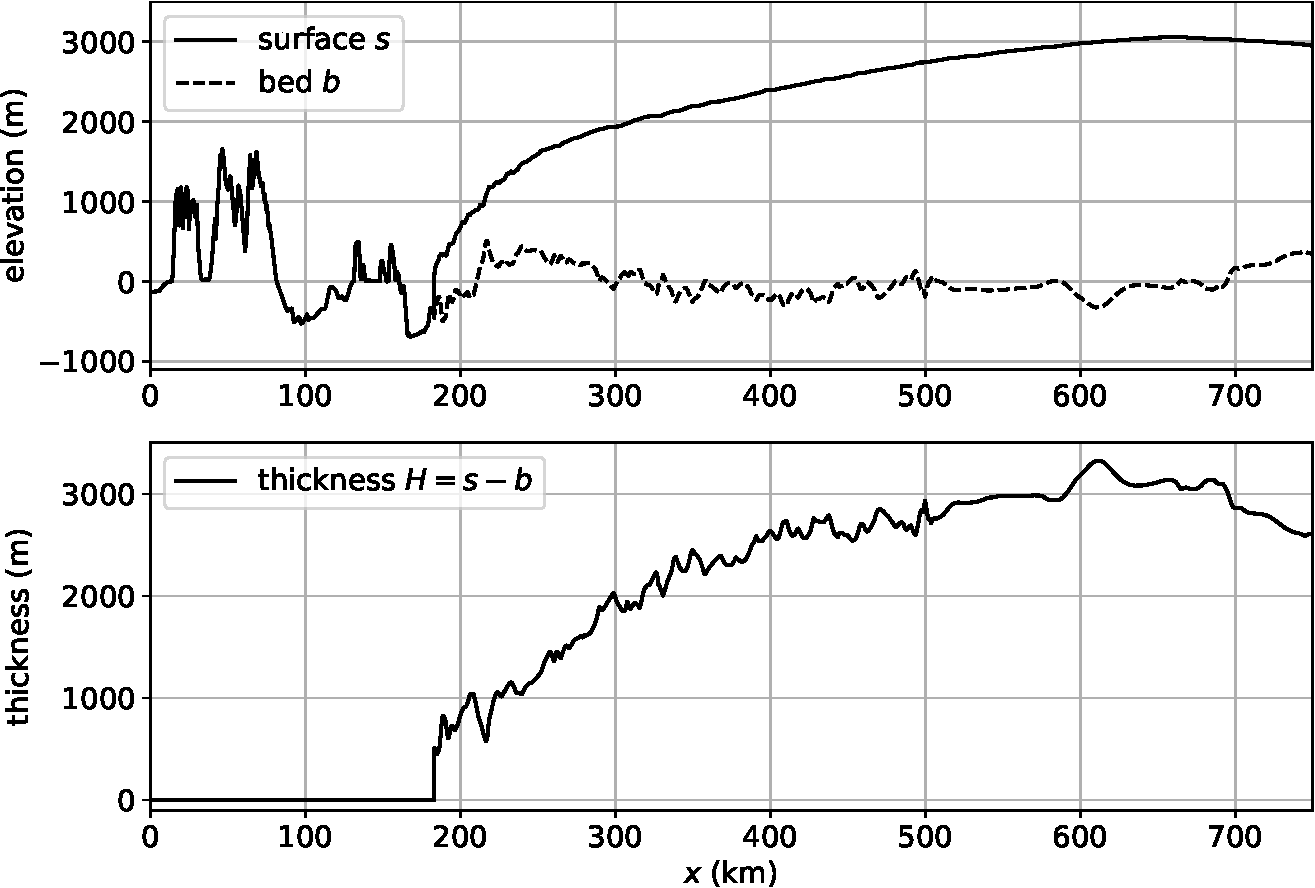
\includegraphics[width=\textwidth]{genfigs/giscross.pdf}
\end{minipage}
\,
\begin{minipage}[t]{0.13\textwidth}
\vspace{10pt}
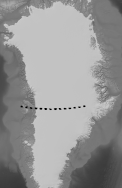
\includegraphics[width=\textwidth]{genfigs/gis/gris-profile-gray.png}
\end{minipage}
\caption{A cross-section of the Greenland ice sheet at $70^\circ$N latitude (inset).  While the ice surface $s$ is relatively smooth because of ice flow (top), the bedrock elevation $b$ is much rougher.  The corresponding ice thickness $H = s-b$ (bottom), though a valid geometry parameterization, inherits the low regularity of $b$.  (Data from \cite{Morlighemetal2017} and A.~Aschwanden, personal communication.)}
\label{fig:giscross}
\end{figure}

FIXME: WHAT WE ACCOMPLISH

This paper is organized as follows.  In Section \ref{sec:model} we reformulate the coupled problem \eqref{eq:icydomain}--\eqref{eq:stokes} as a VI weak form for an implicit (backward Euler) time step.  Well-posedness for this time-step problem is conjectured in Section \ref{sec:theory}, over a Sobolev space of surface elevation functions, and context is provided for this conjecture.  In Section \ref{sec:abstractestimate} we prove an abstract FE error estimate, namely Theorem \ref{thm:abstractestimate} and its corollaries, for general VI problems involving fully-nonlinear, but coercive and Lipshitz, operators on Banach spaces.  This estimate extends the classical case by Falk \cite{Falk1974}, for bilinear forms.  In Section \ref{sec:application} we apply this theorem to the glacier model.  The distinctive character of non-sliding land-based glaciers, regarding how they respond to climate (mass balance) perturbations, and that they stagnate as they approach zero thickness, implies that certain terms are effectively small, and computable geometry error upper bounds follow.  The estimates are demonstrated in Section \ref{sec:demo} on an idealized, but non-trivial, glacier simulation implemented in Firedrake \cite{Hametal2023}.


\section{An implicit time-step model, in weak form} \label{sec:model}

Let $\{t_n\}$ be an increasing sequence of times, and write $\Delta t = t_n-t_{n-1}$ for the step length.  Suppose $s(x)\approx s(t_n,x)$ approximates the unknown surface elevation at time $t_n$.  Let $a^n(x)$ be the (temporal) average of $a(t,x)$ over $[t_{n-1},t_n]$.  Using a backward Euler implicit step \cite{AscherPetzold1998}, SKE \eqref{eq:ske} becomes
\begin{equation}
\frac{s - s^{n-1}}{\Delta t} - \bu|_{s} \cdot \bn_{s} - a^n = 0. \label{eq:be:ske}
\end{equation}
For cleaner appearance we define the source term
\begin{equation}
\ell^n(x) = s^{n-1}(x)+\Delta t\,a^n(x) = s^{n-1}(x) + \int_{t_{n-1}}^{t_n} a(t,x)\,dt. \label{eq:be:source}
\end{equation}
Similar to \eqref{eq:ncp}, the problem is of free-boundary type, and generally $s$ does not solve \eqref{eq:be:ske} over all of $\Omega$.  Instead it solves an NCP:
\begin{subequations}
\label{eq:be:ncp}
\begin{align}
s - b &\ge 0 \label{eq:be:ncp:constraint} \\
s - \Delta t\,\bu|_s \cdot \bn_s - \ell^n &\ge 0 \\
(s - b) \left(s - \Delta t\,\bu|_s \cdot \bn_s - \ell^n\right) &= 0 \label{eq:be:ncp:complementarity}
\end{align}
\end{subequations}
Equation \eqref{eq:be:ncp:complementarity} says that, at the end of the time step $t=t_n$, either there is no ice ($s=b$), or that \eqref{eq:be:ske} holds, almost everywhere over $\Omega$.

The strong form NCP \eqref{eq:be:ncp} has a weak-form variational inequality (VI; \cite{KinderlehrerStampacchia1980}) version which is suited to both well-posedness theory and finite element (FE) analysis.  However, the precise Banach space $\cV$ of surface elevations in this VI is unknown, so for now the space $\cV$ is abstract.  (See Conjecture \ref{conj:wellposed:be} below.)  Admissible surface elevations are from a convex and closed subset of $\cV$:
\begin{equation}
\cK = \left\{r \in\cV\,:\,r \ge b\right\}.  \label{eq:be:admissible}
\end{equation}

We derive the VI form \cite{Bueler2021conservation} as follows, temporarily supposing that $s$ is sufficiently-regular to solve NCP \eqref{eq:be:ncp}.  Let $\Omega_I$ be a (measurable) subset of $\Omega$ on which constraint \eqref{eq:be:ncp:constraint} is inactive, which is to say that glacier ice is present: $\Omega_I \subset \{x\,:\,s(x)>b(x)\}$.  From \eqref{eq:be:ncp:complementarity} it follows by integration that
\begin{equation}
\int_{\Omega_I} \left(s - \Delta t\,\bu|_s \cdot \bn_s - \ell^n\right)\,(r-s) = 0.  \label{eq:inactivetruth}
\end{equation}
for all $r\in\cK$.  On the other hand, suppose $\Omega_A \subset \{x\,:\,s(x)=b(x)\} \subset \Omega$ is a subset of the active (ice-free) region.  Note that $r-s=r-b\ge 0$ on $\Omega_A$ for $r\in\cK$, and observe that $\ell^n - b \le 0$ on $\Omega_A$ because otherwise, assuming continuity of $b$, $s^{n-1}$, and $a^n$, a glacier would still be present (or would have appeared) somewhere in $\Omega_A$, a contradiction.  Using $\bu|_s=0$ on $\Omega_A$, i.e.~velocity extension by zero to all of $\Omega$, and because $b-\ell^n \ge 0$ and $r-s\ge 0$ on $\Omega_A$, integration now yields an inequality:
\begin{equation}
\int_{\Omega_A} \left(s - \Delta t\,\bu|_s \cdot \bn_s - \ell^n\right)\,(r-s) = \int_A \left(b - \ell^n\right)\,(r-b) \ge 0.  \label{eq:activetruth}
\end{equation}
Almost everywhere on $\Omega$, either land is glacier covered ($\Omega_I$) or ice-free ($\Omega_A$), and so the application of \eqref{eq:inactivetruth} or \eqref{eq:activetruth} justifies the following VI model for $s \in \cK$:
\begin{equation}
\int_\Omega \left(s - \Delta t\,\bu|_s \cdot \bn_s\right)\,(r-s) \ge \int_\Omega \ell^n \,(r-s) \quad \text{for all } r \in \cK. \label{eq:be:viearly}
\end{equation}
This integral inequality is meaningful in advance of knowing its solution; it does not require knowledge of the ice-covered part of the domain.
	
Next, for $s\in \cV$ we state the weak form of the Stokes equations \eqref{eq:stokes} on the domain $\Lambda(t_n)$ defined by \eqref{eq:icydomain}, now denoted simply by $\Lambda$.  Note that this Stokes problem computes the field $\bu|_s$ which appears in VI \eqref{eq:be:viearly}.  Here the relevant function spaces are well-known.  Denote by $W^{k,r}(\Lambda)$ the Sobolev space of functions with $k$ weak derivatives which are $r$th-power integrable \cite{Evans2010}.  We will assume that the ice base $\Gamma_b\subset\partial \Lambda$, on which a Dirichlet condition $\bu=\bzero$ holds, has positive measure, and otherwise we suppose that the boundary $\partial \Lambda$ is stress-free.  Recall that $\pp=(1/\nn)+1\approx 4/3$.  Let $W_b^{1,\pp}(\Lambda)^{3}$ be the space of velocity functions which are zero along $\Gamma_b$.  Define
\begin{equation}
\mathcal{M}_\Lambda = W_b^{1,\pp}(\Lambda)^3 \times L^\qq(\Lambda)  \label{eq:mixed}
\end{equation}
as the (mixed) space of admissible velocity and pressure pairs, where $\qq=\pp/(\pp-1)\approx 4$ is the conjugate exponent.  The Glen-Stokes solution $(\bu,p) \in \mathcal{M}_\Lambda$ satisfies the mixed weak form
\begin{equation}
F_\Lambda(\bu,p)[\bv,q] = \int_\Lambda 2 \nu(|D\bu|) D\bu : D\bv - p \Div\bv - (\Div\bu) q - \rhoi \bg \cdot \bv = 0 \label{eq:glenstokesweak}
\end{equation}
for all $(\bv,q) \in \mathcal{M}_\Lambda$.  Recall that the the viscosity $\nu(|D\bu|)$ is defined by \eqref{eq:glen}.

Jouvet and Rappaz \cite{JouvetRappaz2011} prove that \eqref{eq:glenstokesweak} is well-posed under the above assumptions if also the Neumann portion of $\partial\Lambda$ is $C^1$; we return to this regularity concern below.  They show well-posedness via the equivalence of \eqref{eq:glenstokesweak} and minimization of a convex and coercive functional over the divergence-free subspace.  Observe that if the solution to \eqref{eq:glenstokesweak} is sufficiently regular then it satisfies strong equations \eqref{eq:stokes}.

The well-posedness of problem \eqref{eq:glenstokesweak} allows us to create a well-defined map from admissible surface elevations $s$ to the corresponding surface value of the Stokes velocity solution $\bu$.  The map is defined via \eqref{eq:icydomain}, next the solution of \eqref{eq:glenstokesweak} over domain $\Lambda=\Lambda(t)$, and then evaluation of the trace of $\bu$.  This creates the \emph{surface motion map} $\Phi:\cV \to \cV'$, based also on weak derivatives of $s$ to compute $\bn_s$:
\begin{equation}
\Phi(s) = - \bu|_s\cdot \bn_s \label{eq:be:Phidefine}
\end{equation}
For any surface elevation $s$ so that \eqref{eq:glenstokesweak} is well-posed, this map evaluates the dynamical term in SKE \eqref{eq:be:ske}.  Now we can define a final weak form operator $F_{\Delta t}:\cV\to\cV'$:
\begin{equation}
\ip{F_{\Delta t}(s)}{r} = \Delta t\,\ip{\Phi(s)}{r} + \int_\Omega s r = \int_\Omega \left(s - \Delta t\, \bu|_s \cdot \bn_s\right) r.  \label{eq:be:Fdefine}
\end{equation}

At this point, VI problem \eqref{eq:be:viearly} can be re-written using well-defined operators, as follows.  This assumes that $\cV$ has been chosen in an appropriate manner, which requires that the solution surface elevation $s$ is regular enough so that the corresponding Stokes problem is well-posed.  Also we assume, reasonably, that the source term $\ell^n$ defined in \eqref{eq:be:source} is the dual space $\cV'$.  Then we seek $s = s^n \in \cK$ so that
\begin{equation}
\ip{F_{\Delta t}(s)}{r-s} \ge \ip{\ell^n}{r-s} \quad \text{for all } r \in \cK. \label{eq:be:vi}
\end{equation}
This VI form is our preferred weak form associated to the strong-form NCP statement \eqref{eq:be:ncp} of the implicit time step.


\section{Theoretical considerations on the VI problem} \label{sec:theory}

VI problem \eqref{eq:be:vi} is the weak form corresponding to NCP \eqref{eq:be:ncp}.  There is general agreement among glaciologists that, for a non-sliding and isothermal glacier modeled as a very viscous and incompressible fluid, a glacier satisfies the conditions of such an NCP.  For instance, numerical ice sheet models \cite{IsaacStadlerGhattas2015,WirbelJarosch2020} are based upon the Stokes model \eqref{eq:stokes}, and the SKE \eqref{eq:ske} is the standard model for surface geometry evolution \cite{GreveBlatter2009,SchoofHewitt2013}.  The idea that positive and continuous SMB implies the existence at a given location is not controversial.

However, the numerical error bounds proven in Sections \ref{sec:abstractestimate} and \ref{sec:application} depend on a well-posed VI problem for the continuum surface elevation.  Because no results known to this author prove well-posedness for \eqref{eq:be:vi}, nor for any similar glacier geometry problem based on Stokes dynamics, we necessarily conjecture well-posedness (subsection \ref{subsec:conjecture}).  We build up to this conjecture using restricted cases and physical reasoning.

\subsection{Only the first explicit step problem is well-posed} \label{subsec:explicit}   First consider a glacier that does not flow at all.  The glacier geometry time-step problem then reduces to determining the shape of a mere ``snow field'', parameterized by ice-equivalent surface elevation, according only to the SMB and the prior geometry.  The weak form of this problem is well-posed over $L^2(\Omega)$.  In fact, let $\ip{F^{\bzero}_{\Delta t}(s)}{r} = \int_\Omega sr$, which sets $\bu|_s=\bzero$ in definition \eqref{eq:be:Fdefine} of operator $F_{\Delta t}$.  Assuming reasonably that $\ell^n \in (L^2(\Omega))' \cong L^2(\Omega)$---see definition \eqref{eq:be:source}---there exists a unique solution $s^{\bzero} \in \cK_{L^2} = \left\{r\in L^2(\Omega)\,:\,r \ge b\right\}$ of the simplified no-flow VI problem
\begin{equation}
\ip{F^{\bzero}_{\Delta t}(s^{\bzero})}{r-s^{\bzero}} \ge \ip{\ell^n}{r-s^{\bzero}} \quad \text{for all } r \in \cK_{L^2}.
\end{equation}
It is well-known \cite[section II.3]{KinderlehrerStampacchia1980} that the solution of this $L^2$ problem is by truncation:
\begin{equation}
s^{\bzero} = \max\{b, \ell^n\} = \max\{b, s^{n-1} + \Delta t\,a^n\} \in \cK_{L^2}.
\end{equation}
For this problem, a simulation computes $\ell^n$ by straightforward time integration of the SMB $a(t,x)$, and then assesses whether it is admissible, applying pointwise (e.g.~mesh nodal) truncation up to the bed elevation where admissibility is violated ($\ell^n < b$).

The explicit time-step VI problem which corresponds to \eqref{eq:be:vi} has the same character.  Suppose $s^{n-1}$ is admissible and sufficiently regular so that $\bn_{s^{n-1}}$ is well-defined, and so that the weak-form Stokes problem \eqref{eq:glenstokesweak} is well-posed over the domain $\Lambda^{n-1}$ (defined by $s^{n-1}$).  Then define, corresponding to \eqref{eq:be:Fdefine}, the explicit weak form operator:
\begin{equation}
\ip{F^{\text{e}}_{\Delta t}(s)}{r} = \int_\Omega \left(s - \Delta t\, \bu|_{s^{n-1}} \cdot \bn_{s^{n-1}}\right) r.  \label{eq:explicitFdefine}
\end{equation}
This operator arises by replacing the backward Euler SKE equation \eqref{eq:be:ske} with its forward Euler version.  The corresponding VI problem
\begin{equation}
\ip{F^{\text{e}}_{\Delta t}(s^{\text{e}})}{r-s^{\text{e}}} \ge \ip{\ell^n}{r-s^{\text{e}}} \quad \text{for all } r \in \cK_{L^2}
\end{equation}
is again well-posed, and it is solved by truncation \cite[section II.3]{KinderlehrerStampacchia1980}:
\begin{equation}
s^{\text{e}} = \max\{b, s^{n-1} - \Delta t\, \bu|_{s^{n-1}} \cdot \bn_{s^{n-1}} + \Delta t\,a^n\} \in \cK_{L^2}. \label{eq:explicits}
\end{equation}

However, this leaves no regularity for the next step.  The derivatives in $\bn_{s^{n-1}}$, and also the possibility that the velocity trace $\bu|_{s^{n-1}}$ and/or the SMB $a^n$ lack differentiability, imply that $s^{\text{e}}$ defined by \eqref{eq:explicits} is generally not regular enough to serve as the known/previous surface elevation for the next time step.  In particular, it is not clear if $s^{\text{e}}$ defines a domain $\Lambda^{\text{e}}$ over which the (weak) Stokes problem \eqref{eq:glenstokesweak} can be again well-posed.

It is worthwhile to re-state this situation more generously, because explicit time-stepping simulations governed by Stokes dynamics, for glaciers and ice sheets, are common in the applied literature.  There is no \emph{a priori} mathematical reason why these schemes should converge under space-time mesh refinement, because the continuum limit of the time-evolving solution, resulting from taking multiple time steps and refining the spatial mesh, is not even conjecturally clear.  This situation relates closely to current, very incomplete, understanding of which refinement paths for such explicit simulations are conditionally stable \cite[and references therein]{Bueler2023,Chengetal2017,LofgrenAhlkronaHelanow2022}.

\subsection{The problem is not of advection type} \label{subsec:notadv}  It is common in the literature to regard the SKE \eqref{eq:ske} as an advection, based on its appearance,\footnote{Often written $\frac{\partial s}{\partial t} + u \frac{\partial s}{\partial x} + v \frac{\partial s}{\partial y} = a + w$, where $(u,v,w)$ denotes the surface velocity \cite{GreveBlatter2009,SchoofHewitt2013}.} but this is far from the whole truth.  At a simple mathematical level, it is not an advection because the surface velocity appearing in \eqref{eq:ske} is not supplied externally.  Instead the ``advecting velocity'' is itself determined through the simultaneous stress balance equations, on the domain determined by the solution $s$ itself.  At a simple physical level, in a gravity-driven free-surface viscous flow it is clear that the shape responds to local surface perturbations with a negative feedback.  The flow response to a raised bump on the surface tends to remove the bump, and likewise for an indentation in the surface.  In other words, the surface responds diffusively, at least in part, and this substantially explains the smooth appearance of the surface elevation (Figure \ref{fig:giscross}).

For the shallow ice approximation (SIA) this diffusive response is precise.  FIXME state formulas for $u_s,v_s,w_s$ from nonsliding $\nn=3$ SIA; write SKE that results; observe negative feedback response to surface perturbations

Note that well-posedness results are known for such SIA models.  Note that in SIA models the ice geometry often parameterized using the ice thickness.  Using incompressibility, the SKE is replaced by a mass continuity or Saint Venant equation \cite{JouvetBueler2012}, and the corresponding constraint set is $\tilde{\cK} = \{H\ge 0\}$ where $H=s-b$ is the ice thickness.   For the steady SIA model, with arbitrary smooth bed elevations, existence is known.  The existence theorem in \cite{JouvetBueler2012} says that $H$ exists so that its power is in an identified Sobolev space:\footnote{However, the set of functions whose $\rr$th power is in a $W^{1,\qq}$ space is not generally even a vector space.  For example, relevant to the typical powers $\qq=4$ and $\rr=2\qq/(\qq-1)=8/3$ arising from the SIA model for glaciers, and in 1D, if $f(x)=(x-1/2)^{3/8} \chi_{[1/2,1]}(x)$ and $g(x)=1$ then $f^\rr,g^\rr \in W^{1,4}([0,1])$ but $(f+g)^\rr\notin W^{1,4}([0,1])$.} $\eta = H^{2\qq/(\qq-1)} \in W^{1,\qq}(\Omega)$.  See also \cite{Calvoetal2003,PiersantiTemam2023} regarding flat-bed and time-dependent well-posedness results.  On the other hand, the clear diffusion-type solution regularity which occurs in an SIA model likely will not agree with the currently-unknown regularity of a surface elevation solution of \eqref{eq:be:vi} when using non-shallow (Stokes) dynamics.  The wavelength-dependent surface response of the Stokes model has a different small wavelength limit from the diffusive SIA model \cite[for example]{Pattynetal2008}, though this limit is not precisely understood.

\subsection{The problem is not of optimization type} \label{subsec:notopt}  FIXME porous medium character, i.e.~coercivity blocked by thickness (power) scaling of operator; calculation shows weak form op $\ip{F(u)}{v} = F(u)[v] = \int u \grad u\cdot \grad v$ does not have symmetry $F'(u)[v,w] = F'(u)[w,v]$ which would arise if $F(u)=J'(u)$ for objective $J(u) \in \RR$

FIXME physically, thin ice does not flow much regardless of surface slope, which is reflected in $(s-b)^4$ coefficient in surface velocity formula

\subsection{Physical reasoning related to margin/terminus shape} \label{subsec:margin}  FIXME Also, the theoretical shapes of glacier and ice sheet \emph{margins} (Figure \ref{fig:margins}) are not so clear, speaking here of the grounded case.  Margin shape relates to which Sobolev spaces might be credible for claims of well-posedness.  The SIA theory suggests root-type (fractional-power) shapes \cite{Bueleretal2005} with unbounded gradients.  By contrast, earlier glacier modeling often hypothesized a ``wedge'' shape with a finite gradient \cite[for example]{EchelmeyerKamb1986}, which might allow $s\in W^{1,\rr}(\Omega)$.  Reality is of course much more complicated, with fracture, crevasse, and cliffs as common features of glacier margins, while here we assume ice is only modeled as a viscous fluid.

\begin{figure}
\begin{center}
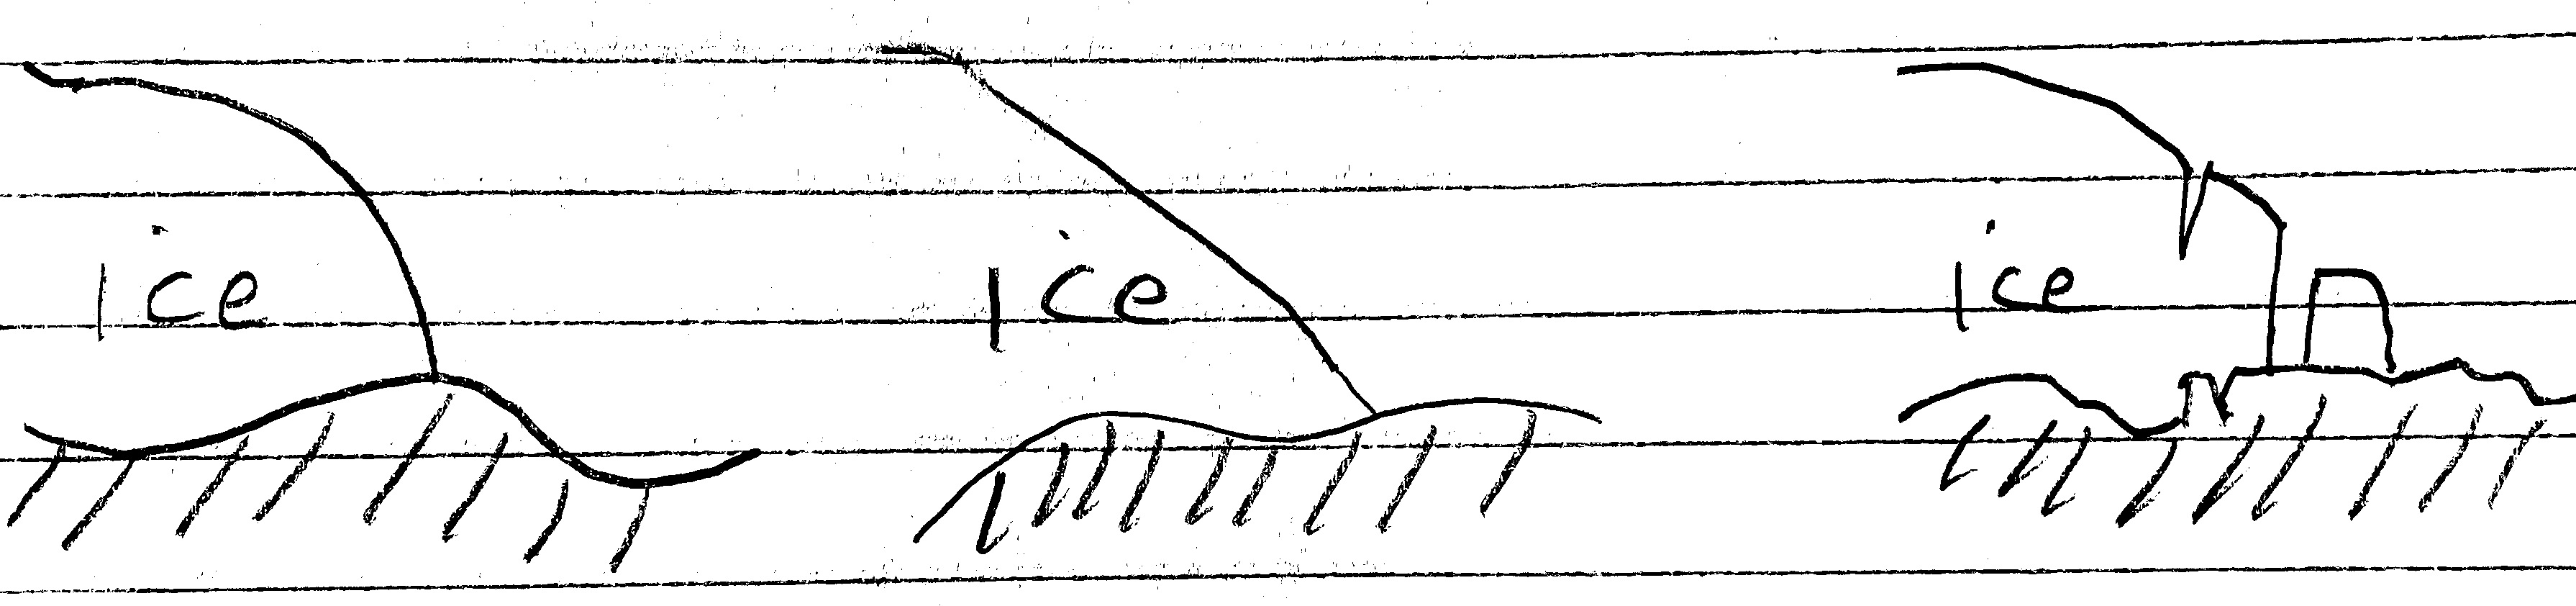
\includegraphics[width=0.8\textwidth]{figs/margins.jpg}
\end{center}
\caption{In which Sobolev space should we seek the surface elevation function?  This question relates to the theoretically-expected shape of the ice margin.  The shallow ice theory yields a fractional power shape (left).  Other glacier models hypothesize a ``wedge'' shape (center).  On the other hand, actual glacier margins often have overhangs, crevasses, and cliffs (right).} %FIXME replace with better figure
\label{fig:margins}
\end{figure}

In the vicinity of a steep ice margin, especially on steep bedrock features, glacier ice can actually generate overhangs which violate the assumption that a surface elevation function is even meaningful.  Overhangs can also occur in the bedrock.  Because such overhangs are small features compared to the overall scale of glaciers and ice sheets, almost all modeling literature ignores their formation and assumes instead that surface and bed elevation functions are well-defined; see \cite{IsaacStadlerGhattas2015,Jouvetetal2008,LofgrenAhlkronaHelanow2022,WirbelJarosch2020} among many examples.  Reference \cite{PralongFunk2005} provides an alternative model in which overhangs are allowed and ice-cliff calving occurs via a damage variable and a stress-fracture failure criterion.  Such a mechanism might explain how (nearly) well-defined surface elevation and thickness functions could arise as solutions in a more-complete, and potentially well-posed, model.  However, such a viscous-brittle model is a highly nontrivial extension of the viscous-only model herein.

\subsection{Conjectural well-posedness for the continuum problem} \label{subsec:conjecture} FIXME transition: subsections \ref{subsec:explicit}--\ref{subsec:margin} deploy imperfect arguments to explain why problem \eqref{eq:be:vi} is the one we should concentrate on, with the understanding that it is non-trivial (i.e.~not just optimization or simple advection either); now we give our best guess

\begin{conjecture} \label{conj:wellposed:be}
There exists an exponent $\rr$ so that if $\cV = W^{1,\rr}(\Omega)$ then, for all sufficiently-small values $\Delta t>0$, there exists a unique solution $s \in \cK = \{r\ge b\} \subset \cV$ to VI problem \eqref{eq:be:vi}.
\end{conjecture}

Conjecture \ref{conj:wellposed:be} addresses the well-posedness of a single implicit time-step problem, and this is not sufficient to show well-posedness of the time-dependent problem.  Without making a further formal conjecture, some versions of the following propositions must be true:
\renewcommand{\labelenumi}{\emph{\roman{enumi})}}
\begin{enumerate}
\item The solution $s$ of \eqref{eq:be:vi} is sufficiently regular so that $\ell^{n+1} \in \cV'$ is well-defined for the next step.
\item The parabolic VI problem \cite{Glowinski1984} corresponding to time-dependent NCP \eqref{eq:ncp} is well-posed.
\end{enumerate}
While practitioners of numerical ice sheet and glacier modeling using Stokes dynamics expects facts like these to hold, they may be distant mathematically despite progress in the SIA case, especially on \emph{ii)} \cite{Calvoetal2003,PiersantiTemam2023}.  On the other hand, the results in the next two Sections only require Conjecture \ref{conj:wellposed:be}.


\section{Abstract error estimate} \label{sec:abstractestimate}

We now consider the FE approximation of an abstract variational inequality (VI) problem.  We will return to \eqref{eq:be:vi} in Section \ref{sec:application}.

Let $\cV$ be a real reflexive Banach space with norm $\|\cdot\|$ and topological dual space $\cV'$.  Denote the dual pairing of $\phi \in \cV'$ and $v\in\cV$ by $\ip{\phi}{v} = \phi(v)$, and define the (Banach space) norm on $\cV'$ by $\|\phi\|_{\cV'} = \sup_{\|v\|=1} |\!\ip{\phi}{v}\!|$.  Let $\cK \subset \cV$ be a nonempty, closed, and convex subset, the constraint set; elements are said to be admissible.  For a continuous, but generally nonlinear, operator $f:\cK \to \cV'$, and a linear source $\ell\in \cV'$, the VI problem is to find $u\in \cK$ such that
\begin{equation}
\ip{f(u)}{v-u} \ge \ip{\ell}{v-u} \quad \text{for all } v\in \cK. \label{eq:vi}
\end{equation}
The best known example of such a problem is the obstacle problem for the Laplacian operator; see \cite{Ciarlet2002,Evans2010,KinderlehrerStampacchia1980} for its theory and FE analysis.

The following definitions are standard \cite[Chapter III]{KinderlehrerStampacchia1980}.

\begin{definition} \label{def:monotonepcoercive}
An operator $f:\cK \to \cV'$ is said to be \emph{monotone} if
\begin{equation}
\ip{f(v)-f(w)}{v-w} \ge 0 \qquad \text{for all } v,w \in \cK \label{eq:monotone}
\end{equation}
and \emph{strictly monotone} if equality in \eqref{eq:monotone} implies $v=w$.  It is \emph{coercive} if there is $w\in \cK$ so that for $v \in \cK$,
\begin{equation}
\frac{\ip{f(v)-f(w)}{v-w}}{\|v-w\|} \to +\infty \qquad \text{as } \|v\| \to +\infty. \label{eq:coercive}
\end{equation}
Let $\pp>1$.  The operator is \emph{$\pp$-coercive \cite{Bueler2021conservation}} if there exists $\alpha>0$ such that
\begin{equation}
\ip{f(v)-f(w)}{v-w} \ge \alpha \|v-w\|^\pp \qquad \text{for all } v,w \in \cK. \label{eq:pcoercive}
\end{equation}
\end{definition}

It is well-known that if $f:\cK \to \cV'$ is monotone and coercive, and also continuous on finite-dimensional subspaces, then VI \eqref{eq:vi} has a solution \cite[Corollary III.1.8]{KinderlehrerStampacchia1980}.  If $f$ is strictly monotone then a solution is unique.  If $f$ is $\pp$-coercive then it coercive and strictly monotone; $\pp$-coercivity and continuity yield well-posedness for \eqref{eq:vi}.
% \cite{Peral1997} uniform continuity over bounded sets for p-Laplacian: Thm A.0.6

\begin{definition} \label{def:lipshitz}
For $\rho>0$ let $B_\rho = \{v\in \cV\,:\,\|v\|\le \rho\}$.  We say $f:\cK \to \cV'$ is \emph{Lipshitz on bounded subsets of $\cK$} if for every $\rho>0$ there is $C(\rho)>0$ so that if $v,w \in B_\rho \cap \cK$ and $z\in\cV$ then $|\ip{f(v)-f(w)}{z}| \le C(\rho) \|v-w\| \|z\|$, equivalently
\begin{equation}
\|f(v)-f(w)\|_{\cV'} \le C(\rho) \|v-w\| \quad \text{ for all } v,w \in B_\rho \cap \cK.  \label{eq:liponbounded}
\end{equation}
\end{definition}

Clearly, if $f$ is Lipshitz on bounded subsets then $f$ is continuous.  Definitions \ref{def:monotonepcoercive} and \ref{def:lipshitz} do not require $f$ to be defined on all of the vector space $\cV$, but only on $\cK$.

A key concept in the following theorem is that $f(u)-\ell$ is generally nonzero when $u$ solves \eqref{eq:vi}.  Instead, a nonlinear complementarity problem holds, at least in sufficiently regular cases, as in \cite[Exercise 5.1.1]{Ciarlet2002}  and \cite[section 7]{BuelerFarrell2024}, for example.  Only for $u$ in the interior of $\cK$ should we expect equality (i.e.~$f(u)=\ell$).

The FE method solves a finite-dimensional VI problem, otherwise comparable to \eqref{eq:vi}.  Suppose $\cV_h \subset \cV$ is a finite-dimensional subspace; typically $\cV_h$ consists of piecewise-polynomial and continuous functions defined on a mesh.  Define the FE constraint set $\cK_h\subset \cV_h$.  In general $\cK_h \nsubseteq \cK$, and no such assumption is made in Theorem \ref{thm:abstractestimate} below.  Let $f_h:\cK_h\to\cV'$.  Generally $f_h\ne f$, because of quadrature and other approximations, and again the general case is considered below.  The FE VI problem is
\begin{equation}
\ip{f_h(u_h)}{v_h-u_h} \ge \ip{\ell}{v_h-u_h} \quad \text{for all } v_h\in \cK_h. \label{eq:fe:vi}
\end{equation}
We assume that $f_h$ is $\pp$-coercive, and thus this problem is also well-posed.

The following abstract error estimate extends \cite{Falk1974} and Theorem 5.1.1 in \cite{Ciarlet2002}.  Here we do not assume that $f$ is linear, nor that $f_h=f$, and $f_h$ need only be defined on $\cK_h$.  However, we must extend the domain of $f$ to include the finite element solution.

\begin{theorem} \label{thm:abstractestimate}  Suppose $u\in\cK$ solves \eqref{eq:vi} and $u_h\in\cK_h$ solves \eqref{eq:fe:vi}.  Define
\begin{equation}
\hcK = \overline{\Hull{(\cK \cup \cK_h)}}  \label{eq:convexhull}
\end{equation}
as the closure in $\cV$ of the convex hull of $\cK \cup \cK_h$, and suppose that $f$ can be extended to $\hcK$.  For $1<\pp<\infty$ assume $f$ is $\pp$-coercive over $\hcK$ with constant $\alpha>0$, and that it is Lipshitz on bounded sets of $\hcK$.  Let $R_h=\max\{\|u\|,\|u_h\|\}$.  Then there is a constant $c=c(\alpha,R_h)>0$ so that
\begin{align}
\|u-u_h\|^p &\le \quad \frac{2}{\alpha} \inf_{v\in\cK} \ip{f(u)-\ell}{v-u_h} \label{eq:abstractestimate} \\
   &\quad + \frac{2}{\alpha} \inf_{v_h\in\cK_h} \ip{f(u)-\ell}{v_h-u} \notag \\
   &\quad + \frac{2}{\alpha} \ip{f(u_h)-f_h(u_h)}{u_h} \notag \\
   &\quad + \inf_{v_h\in\cK_h} c \|v_h - u\|^\qq \notag
\end{align}
\end{theorem}

\begin{proof}  Consider arbitrary elements $v\in\cK$ and $v_h\in\cK_h$.  Rewrite VIs \eqref{eq:vi} and \eqref{eq:fe:vi}, as follows:
\begin{align*}
\ip{f(u)}{u}     &\le \ip{f(u)}{v} + \ell(u-v),  \\
\ip{f_h(u_h)}{u_h} &\le \ip{f_h(u_h)}{v_h} + \ell(u_h-v_h).
\end{align*}
It follows from $\pp$-coercivity over $\hcK$ and these inequalities that
\begin{align*}
\alpha \|u-u_h\|^\pp &\le \ip{f(u)-f(u_h)}{u-u_h} \\
  &= \ip{f(u)}{u} + \ip{f(u_h)}{u_h} - \ip{f(u)}{u_h} - \ip{f(u_h)}{u} \\
  &= \ip{f(u)}{u} + \ip{f_h(u_h)}{u_h} \\
  &\qquad - \ip{f(u)}{u_h} - \ip{f(u_h)}{u} + \ip{f(u_h)-f_h(u_h)}{u_h} \\
  &\le \ip{f(u)}{v} + \ell(u-v) + \ip{f(u_h)}{v_h} + \ell(u_h-v_h) \\
  &\qquad - \ip{f(u)}{u_h} - \ip{f(u_h)}{u} + \ip{f(u_h)-f_h(u_h)}{u_h} \\
  &= \ip{f(u)}{v-u_h} - \ell(v-u_h) + \ip{f(u_h)}{v_h-u} - \ell(v_h-u) \\
  &\qquad + \ip{f(u_h)-f_h(u_h)}{u_h} \\
  &= \ip{f(u)-\ell}{v-u_h} + \ip{f(u)-\ell}{v_h-u} \\
  &\qquad + \ip{f(u)-f(u_h)}{u-v_h} + \ip{f(u_h)-f_h(u_h)}{u_h}
\end{align*}
Since $u,u_h\in B_{R_h}$, by the Lipshitz assumption over $\hcK$ there is $C(R_h)>0$ so that
    $$\ip{f(u)-f(u_h)}{u-v_h} \le C(R_h) \|u-u_h\|\|u-v_h\|.$$
Noting $1<\pp,\qq<\infty$, now use Young's inequality with $\eps>0$ \cite[Appendix B.2]{Evans2010}:
\begin{align*}
\alpha \|u-u_h\|^\pp &\le \ip{f(u)-\ell}{v-u_h} + \ip{f(u)-\ell}{v_h-u} \\
  &\qquad + C(R_h) \left(\eps\|u-u_h\|^\pp + \tilde C(\eps) \|u-v_h\|^\qq\right) + \ip{f(u_h)-f_h(u_h)}{u_h}
\end{align*}
(Here $\tilde C(\eps) = (\eps \pp)^{-\qq/\pp} \qq^{-1}$.)  Choose $\eps>0$ so that $C(R_h) \eps \le \alpha/2$, and subtract:
\begin{align*}
\frac{\alpha}{2} \|u-u_h\|^\pp &\le \ip{f(u)-\ell}{v-u_h} + \ip{f(u)-\ell}{v_h-u} \\
  &\qquad + C(R_h) \tilde C(\eps) \|u-v_h\|^\qq + \ip{f(u_h)-f_h(u_h)}{u_h}
\end{align*}
Take infimums to show \eqref{eq:abstractestimate}.
\end{proof}

Although $f(u)-\ell\in \cV'$ is abstract in Theorem \ref{thm:abstractestimate}, in practical applications it might be a signed measure or even a measurable function.  In such cases, the first two terms in estimate \eqref{eq:abstractestimate} retain information about the sign of $f(u)-\ell$.  By contrast, the original Hilbert space result in \cite{Falk1974} (and \cite[section 5.1]{Ciarlet2002}) compute a norm and lose this information.  Also, these results assume $f_h=f$.  To give the analogous Banach space estimate, as a corollary to Theorem \ref{thm:abstractestimate}, suppose that $\cV$ continuously and densely embeds in a larger Banach space $\cB$:
\begin{equation}
\cV \hookrightarrow \cB, \quad \overline{\cV} = \cB \label{eq:VembedsinB}
\end{equation}
Observe that $\cB' \subset \cV'$.  A standard example is where $\cV=W^{1,\qq}(\Omega)$ and $\cB=L^\qq(\Omega)$.  The proof of the following is immediate.

\begin{corollary}  \label{cor:abstractestimate:Bnorm}  In addition to the assumptions of Theorem \ref{thm:abstractestimate}, suppose that \eqref{eq:VembedsinB} holds, that $f(u_h)=f_h(u_h)$, and that $\|f(u)-\ell\|_{\cB'} < \infty$.  Then
\begin{align}
\|u-u_h\|^\pp &\le \frac{2}{\alpha} \|f(u)-\ell\|_{\cB'} \left( \inf_{v\in\cK} \|v-u_h\|_{\cB} +   \inf_{v_h\in\cK_h} \|v_h-u\|_{\cB} \right) \label{eq:abstractestimate:Bnorm} \\
   &\qquad + \inf_{v_h\in\cK_h} c \|v_h - u\|^\qq \notag
\end{align}
\end{corollary}

On the other hand, the convex hull operation \eqref{eq:convexhull} is not needed if the nonlinear operator $f=f_h$ is defined on all of $\cV$.  That is, \eqref{eq:abstractestimate} obviously holds if one replaces $\hcK$ with $\cV$ itself for the domain of $f$.  Furthermore, for \emph{linear} operators defined in this way, Theorem \ref{thm:abstractestimate} reduces to the FE error estimate for VIs by Falk \cite{Falk1974}.  Specifically, suppose $\ip{f(v)}{w}=a(v,w)$ is actually bilinear, $\cV$-elliptic, and continuous on a Hilbert space $\cV$.  Define $A:\cV\to\cV'$, a bounded linear operator, by $Av(w) = a(v,w)$.  Observe that continuity for $a(v,w)$ implies Lipshitz on bounded sets \eqref{eq:liponbounded} for $A$.  Suppose that $\cV\hookrightarrow \cH$ and $\overline{\cV} = \cH$ for some larger Hilbert space $\cH$, and that $\|Au-\ell\|_{\cH'} < \infty$ so that, up to isomorphism, $Au-\ell \in \cH$.  Then Corollary \ref{cor:abstractestimate:Bnorm} reduces to Theorem 1 in \cite{Falk1974} and Theorem 5.1.1 in \cite{Ciarlet2002}.

As observed in \cite{Ciarlet2002}, the quantity in estimates \eqref{eq:abstractestimate} and \eqref{eq:abstractestimate:Bnorm} which involves $v-u_h$, for $v\in\cK$, is generally nonzero in obstacle problems where $\cK_h \nsubseteq \cK$.  (This is relevant to glacier models tracking the surface elevation, as opposed to thickness.)  In fact, suppose $\cK=\{v \in \cV\,:\,v\ge \psi\}$, $\psi_h$ is an interpolant of $\psi$, and $\cK_h=\{v_h \in \cV_h\,:\,v_h\ge \psi_h\}$.  Observe that, while $\psi_h(x_j)=\psi(x_j)$ for interpolation nodes $x_j$, generally $\psi_h(x) \ge \psi(x)$ does not hold for all $x\in\Omega$, even if $\psi$ is arbitrarily smooth.  In other words, nodal admissiblity does not imply admissibility (Figure \ref{fig:nonadmissible}).

\begin{figure}
\begin{center}
FIXME figure like Ciarlet Figure 5.1.3 %\includegraphics[width=0.8\textwidth]{figs/xxx.jpg}
\end{center}
\caption{Nodal admissibility generally does not imply admissibility.  Thus, if $\phi_h$ is the FE interpolant of an obstacle $\psi$, it is possible that $\cK_h \nsubseteq \cK$.}
\label{fig:nonadmissible}
\end{figure}

The following corollary is relevant to glacier models solving for ice thickness, as opposed to surface elevation.  In such cases $\cK = \{v\ge 0\}$ consists of all nonnegative functions and $\cK_h=\cK\cap\cV_h$.

\begin{corollary}  \label{cor:abstractestimate:subset}  Keeping the assumptions of Theorem \ref{thm:abstractestimate}, suppose also that $\cK_h \subset \cK$, and that $f(u_h)=f_h(u_h)$.  Then
\begin{equation}
\|u-u_h\|^\pp \le  \inf_{v_h\in\cK_h} \left\{\frac{2}{\alpha} \ip{f(u)-\ell}{v_h-u} + c \|v_h - u\|^\qq\right\}. \label{eq:abstractestimate:subset}
\end{equation}
If also the assumptions of Corollary \ref{cor:abstractestimate:Bnorm} hold then
\begin{equation}
\|u-u_h\|^\pp \le \inf_{v_h\in\cK_h} \left\{\frac{2}{\alpha} \|f(u)-\ell\|_{\cB'} \|v_h-u\|_{\cB} + c \|v_h-u\|^\qq\right\} \label{eq:abstractestimate:subset:Bnorm}
\end{equation}
Finally, if additionally $f(u)=\ell$ then
\begin{equation}
\|u-u_h\| \le \tilde c \inf_{v_h\in\cK_h} \|v_h-u\|^{\qq/\pp} \label{eq:abstractestimate:subset:Cea}
\end{equation}
\end{corollary}

Regarding \eqref{eq:abstractestimate:subset:Cea}, which is Cea's lemma \cite[Theorem 2.4.1]{Ciarlet2002} translated to Banach spaces, $f(u)=\ell$ would be true if $u$ were in the interior of $\cK$, with no free boundary or active set.  Said another way, in \eqref{eq:abstractestimate:subset:Cea} we have reduced to the PDE case.  In the glacier context, to which we return now, \eqref{eq:abstractestimate:subset:Cea} corresponds to the case where the entire domain $\Omega$ is covered in ice.


\section{Application of the estimate} \label{sec:application}

FIXME apply Theorem \ref{thm:abstractestimate} and talk through what happens

FIXME accomodate the barrier theory from \cite{Bueler2021conservation}


\section{Demonstration of computable geometry error bounds} \label{sec:demo}

FIXME use stuff from multilevel-stokes-geometry


\section{Conclusion} \label{sec:conclusion}

FIXME


\bibliographystyle{siamplain}
\bibliography{estimate}

\end{document}
